\documentclass{article}

\usepackage{style/preamble}
\usepackage{style/mytikz}
\usepackage{parskip}

\newcounter{dip}

\begin{document}
  \title{Problem Set 2 - Ramification}
  \date{}
  \maketitle









\section{Meromorphic functions on $\bbp^1$}

The last step in completing the proof of the theorem that proves that all meromorphic functions on $\bbp^1$ are rational functions is the following.

Let $f: \bbp^1 \rightarrow \bbp^1$ be a meromorphic function.
Let $\calz = f^{-1}(0) \cap \bbc$ and $\calp = f^{-1}(\infty) \cap \bbc$. (I had forgotten to add ``$\cap \bbc$'' last time. This is necessary as we do not know how to multiply or divide by $\infty$.)
The elements of $\calz$ are the zeroes and the elements of $\calp$ are the poles of $f$ inside $\bbc$.

\begin{proposition}
  \label{thm:Theorem1}
  The function
  \begin{align*}
    g(z) = f(z) \cdot \dfrac{(z-p_1)^{k_1} \dots (z-p_n)^{k_n}}{(z-z_1)^{\ell_1} \dots (z-z_m)^{\ell_m}}
  \end{align*}
  is meromorphic and has no zeroes or poles in $\bbc$, for some positive integers $k_1, \dots, k_n$ and $\ell_1, \dots, \ell_m$.
\end{proposition}

The proof is by induction on $m + n$. If $m + n = 0$ i.e. there are no poles or zeroes in $\bbc$ we are done.

\begin{definition}
  The order of a zero $z_i$ is the smallest positive integer $k$ such that the $k^{th}$ derivative $f^{(k)}(z_i)$ does not equal $0$.
\end{definition}

\begin{definition}
  The order of a pole $p_i$ is the smallest positive integer $\ell$ such that the $\ell^{th}$ derivative $(f \circ \varphi_2^{-1})^{(\ell)}(p_i)$ does not equal $0$.
\end{definition}



\begin{qbox}
  Suppose $f(z)$ has a zero $z_i$ of order $k$. Show that
  \begin{align*}
    g(z) = \begin{cases}
        \dfrac{f(z)}{(z - z_i)^k} & \mbox{ if }z \neq z_i \\
        \lim \limits_{z \rightarrow z_i} \dfrac{f(z)}{(z - z_i)^k} & \mbox{ if } z = z_i
    \end{cases}
  \end{align*}
  has no zero at $z_i$.\hint{Look at the Taylor series expansion of $f$ at $z_i$.}
  Further argue that the set of zeroes and poles of $g(z)$ in $\bbc$ are $\calz \setminus \set{z_i}$ and $\calp$, respectively.
\end{qbox}


\begin{qbox}
  Suppose $f(z)$ has a pole $p_i$ of order $\ell$. Show that
  \begin{align*}
    g(z) = \begin{cases}
        f(z) (z - p_i)^\ell & \mbox{ if }z \neq p_i \\
        \lim \limits_{z \rightarrow p_i} f(z) (z - p_i)^\ell & \mbox{ if } z = p_i
    \end{cases}
  \end{align*}
  has no pole at $p_i$.\hint{Look at the Taylor series expansion of $f \circ \varphi_2^{-1}$ at $\varphi_2(p_i)$.}
  Further argue that the set of zeroes and poles of $g(z)$ in $\bbc$ are $\calz$ and $\calp \setminus \set{p_i}$, respectively.
\end{qbox}

\begin{qbox}
  Complete the proof of Proposition \ref{thm:Theorem1}.
\end{qbox}

Once we see that $g(z)$ has no zeroes or poles in $\bbc$, the only zero or pole of $g(z)$ can be at $\infty$. But $\infty$ can be either a zero or a pole but not both.
Hence the image of $g(z)$ is not surjective. By the exercises, from yesterday $g(z)$ is a constant.











\section{Riemann Surfaces}
\begin{definition}
  A \emph{Riemann surface} is a (nice) topological spaces $X$ along with
  \begin{enumerate}
    \item a covering of open sets
    \begin{align*}
      X = U_1 \cup U_2 \cup \dots
    \end{align*}
    \item continuous injections $\varphi_i: U_i \rightarrow \bbc$ for each $U_i$ in the open cover. (We need injectivity to make sense of $\varphi_i^{-1}$.)
    \item A condition on the \emph{transition functions}.
  \end{enumerate}
  The pair $(U_i, \varphi_i: U_i \rightarrow \bbc)$ is called a \emph{chart} and the collection of charts $\set{(U_i, \varphi_i)}$ is called an \emph{atlas}.
  A \emph{Riemann surface} is a \emph{complex manifold of dimension 1}.
\end{definition}

To understand what the third condition should be we need to understand maps between Riemann surfaces.

\begin{definition}
  A continuous map $f:X \rightarrow Y$ between two Riemann surfaces $X$ and $Y$ with atlases $(U_i, \varphi_i)$ and $(V_j, \psi_j)$, respectively, is \emph{complex differentiable} if
  \begin{align*}
    \psi_j \circ f \circ \varphi_i^{-1}
  \end{align*}
  (appropriately restricted) is holomorphic at $z$ whenever $z \in U_i$ and $f(z) \in V_j$.
\end{definition}

Because the open sets $U_i$ cover $X$ many of these will intersect.
\begin{definition}
  For a Riemann surface $X$ with an atlas $\set{(U_i, \varphi_i)}$, the functions $\varphi_i \circ \varphi_j^{-1}$ are called the \emph{transition} functions or the \emph{change of coordinate} functions.
\end{definition}

Note that the domain of $\varphi_i \circ \varphi_j^{-1}$ is $\varphi_j(U_i \cap U_j)$ and the codomain is $\varphi_i(U_i \cap U_j)$.


\begin{qbox}
  Show that the identity function $\id: X \rightarrow X$ is complex differentiable if and only if all the transition functions are holomorphic.
\end{qbox}

We DO want the identity function to be complex differentiable, which then becomes the third condition in the definition of a Riemann surface:
\begin{enumerate}
  \item[3.] All the transition functions $\varphi_i \circ \varphi_j^{-1}$ are holomorphic.
\end{enumerate}

\begin{qbox}
  Check that the transition functions for $\bbp^1$ are holomorphic.
\end{qbox}

We can think of a function between Riemann surfaces as being a ``piece-wise function'' built by gluing holomorphic functions. Thus, understanding the local structure of complex differentiable functions between Riemann surfaces is equivalent to understanding the local structure of holomorphic functions. On the other hand, understanding the global structure of maps between Riemann surfaces is a much harder question and lies at the heart of complex geometry.






\section{Ramification}
Consider the function \begin{align*}
  f(z) = \dfrac{z^2}{z+1}
\end{align*}
We can solve $ \dfrac{z^2}{z+1} = w $ to see that
\begin{align*}
  z = \dfrac{w \pm \sqrt{w^2 + 4z}}{2}
\end{align*}
For $w \neq 0, -4, \infty$ $f^{-1}(z)$ consists of two points $\set{\dfrac{w + \sqrt{w^2 + 4z}}{2}, \dfrac{w - \sqrt{w^2 + 4z}}{2}}$.
Even for $\infty$, we see that $f^{-1}(\infty) = \set{\infty, -1}$.
But for 0 and 4 we get $f^{-1}(0) = \set{0}$, $f^{-1}(-4) = \set{-2}$.

It is even easier to see this phenomenon for
\begin{align*}
  f(z) = z^n
\end{align*}
In this case every point except $0$ and $\infty$ have exactly $n$ pre-images. We can imagine $z^n$ as the Riemann sphere winding around itself $n$ times.

\begin{definition}
  A continuous map $f: X \rightarrow Y$ between topological spaces is called a (finite) \emph{ramified covering (or a branched covering)} of order $n$ if there exists an isolated collection of points $\set{z_i} \subseteq Y$ such that $f$ restricted to the complement $X \setminus \set{z_i}$ is an $n:1$ map. (To be very precise, we require the restricted map $f|_{X \setminus \set{z_i}}$ to be a covering map.)

  If $f$ is an $n:1$ ramified covering and $w \in Y$ is a point such that $|f^{-1}(w)| \neq n$ we say that $w$ is a \emph{branch point} and the points in $f^{-1}(w)$ are called the \emph{ramified points}.
  The set of all branch points is called the \emph{branch locus} (subset of $Y$) and the set of all ramified points is called the \emph{ramification locus} (subset of $X$).
\end{definition}

\begin{qbox}
  Find the branch and ramification loci in the two examples given above.
\end{qbox}

\begin{qbox}
  \textbf{Fact:} The cubic $x^3 + px + q = 0$ has repeated roots if and only if the discriminant $\Delta = – 4p^3 – 27q^2$ is 0.

  Find the branch and ramification loci of the following function
  \begin{align*}
    f: \bbp^1 &\longrightarrow \bbp^1 \\
    z &\longmapsto z^3 - 3 z
  \end{align*}
\end{qbox}
We are missing one more piece of the story, the ramification index. But for this we need to understand holomorphic functions better.















\section{Local structure of holomorphic functions}
\begin{theorem}
  \label{thm:LocalStructure}
  For an open subset $U \subseteq \bbc$, let $f: U \rightarrow \bbc$ be a non-constant holomorphic function and let $z_0 \in U$.
  Suppose the Taylor series of $f$ near $z_0$ is
  \begin{align*}
    f(z) - f(z_0) = a_k (z - z_0)^k + a_{k+1} (z - z_0)^{k+1} + a_{k+2} (z - z_0)^{k+2} + \dots
  \end{align*}
  with $a_k \neq 0$.
  Then there exists a biholomorphic function $g(z)$ defined in a neighborhood of $f(z)$ such that
  \begin{align*}
    g \circ f (z) = a_k(z - z_0)^k
  \end{align*}
\end{theorem}
\todo[inline]{The statement of this theorem is wrong. Corrected in PSet04.}
\begin{proof}[``Proof'']
  \begin{align*}
    f(z) - f(z_0)
    &=
    a_k (z - z_0)^k + a_{k+1} (z - z_0)^{k+1} + a_{k+2} (z - z_0)^{k+2} + \dots \\
    &=
    a_k (z - z_0)^k \left(1 + \dfrac{a_{k+1}}{a_k} (z - z_0) + \dfrac{a_{k+2}}{a_k} (z - z_0)^{2} + \dots \right) \\
    &\approx a_k (z - z_0)^k
  \end{align*}
  we are done by engineer's induction.
  $g$ is the inverse of the function $1 + \dfrac{a_{k+1}}{a_k} (z - z_0) + \dfrac{a_{k+2}}{a_k} (z - z_0)^{k+2} + \dots $.
\end{proof}

  \begin{definition}
    The $k$ in Theorem \ref{thm:LocalStructure} is called the \emph{ramification index} of $f$ at $z_0$, denoted
    \begin{align*}
      \mathrm{index}_{f}(z_0) = k.
    \end{align*}
  \end{definition}

  \begin{qbox}
    Show that the $\mathrm{index}_{f}(z_0)$ is the smallest integer $k > 0$ such that $f^{(k)}(z_0) \neq 0$, where $f^{(k)}$ denotes the $k^{th}$ derivative.
  \end{qbox}

  \begin{qbox}
    Find the ramification indices of all the points in $\bbc$ for the function $f(z) = z^n$.
  \end{qbox}

  \begin{qbox}
    Use the notation in Theorem \ref{thm:LocalStructure} and restrict $f$ to a sufficiently small neighborhood $V$ and consider $f: V \rightarrow f(V)$.
    Use the previous problem to answer the following.
    \begin{enumerate}
      \item Show that $f$ is a ramified covering of order $k$.
      \item Show that if $k = 1$ then there are no ramification points and if $k > 1$ then the only ramification point is $z_0$.
    \end{enumerate}
  \end{qbox}
  \begin{qbox}
    Let $f: U \rightarrow f(U) \subseteq \bbc$ be a holomorphic function.
    \begin{enumerate}
      \item Show that ramification and branch loci of $f$ are isolated.
      \item Show that if $U$ is compact then the ramification and branch loci of $f$ are finite.
    \end{enumerate}
  \end{qbox}

  \begin{qbox}
    Find the ramification indices of all the points in $\bbc$ for the two examples in the previous section.
  \end{qbox}

  \begin{definition}
    For a non-constant holomorphic function $f: U \rightarrow \bbc$ define the total degree at $w \in \bbc$
    \begin{align*}
      \mathrm{deg}_f(w) = \sum_{z \in f^{-1}(w)} \mathrm{index}_f(z).
    \end{align*}
  \end{definition}

  \begin{qbox}
    Find the total degrees of all the points in $\bbc$ for the function $f(z) = z^n$.
  \end{qbox}

  \begin{qbox}
    Find the total degrees of all the points in $\bbc$ for the two examples in the previous section.
  \end{qbox}

  We will next extend these definitions to all maps between Riemann surfaces.











  \begin{figure}[t]
  \centering
    % \includegraphics[width=0.5\textwidth]{example-image}
    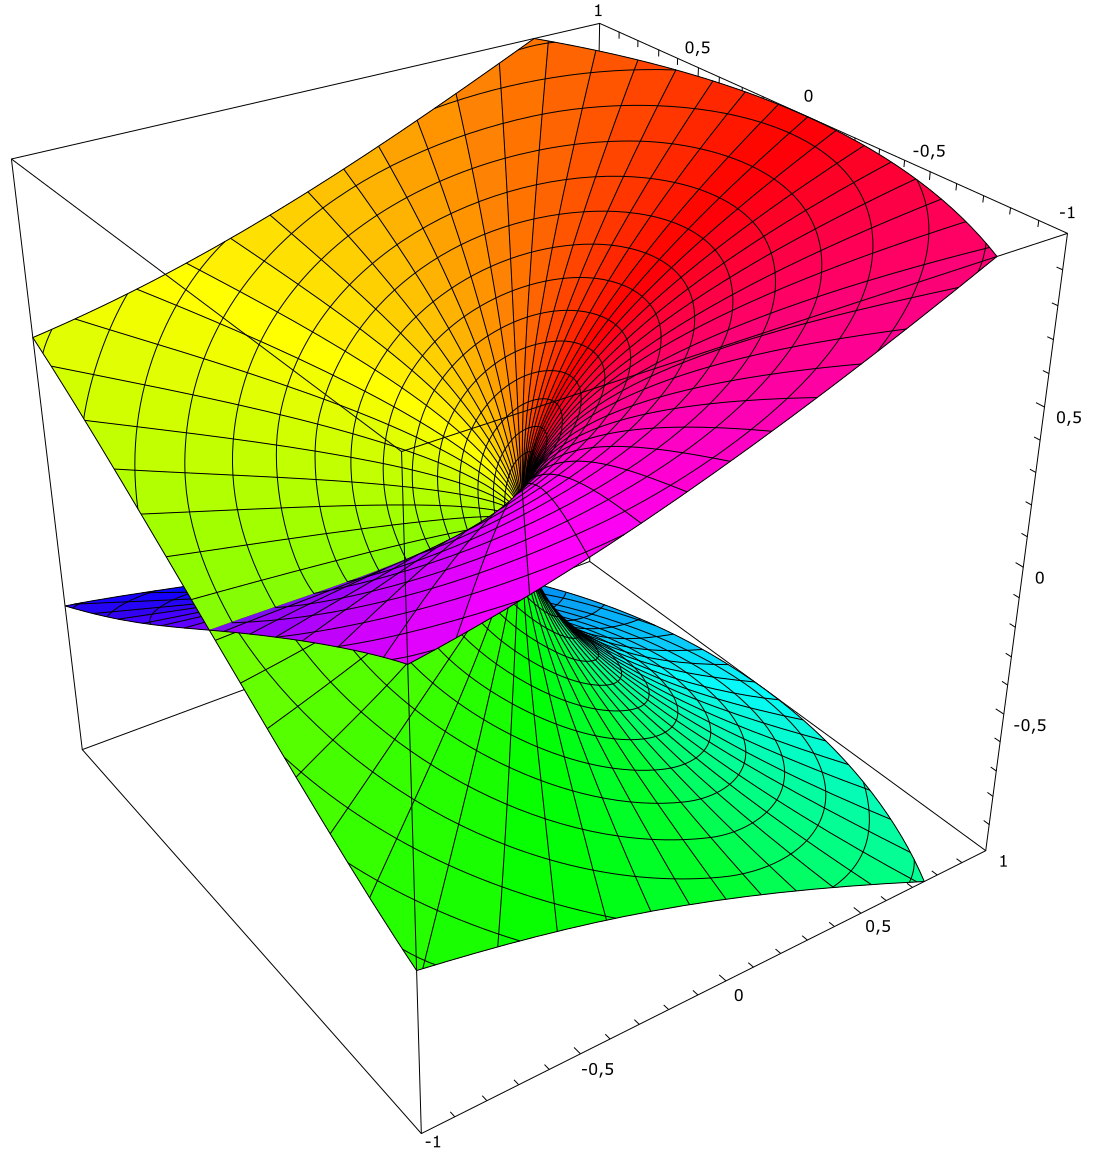
\includegraphics[width=0.4\textwidth]{images/sqrt.png}
    \hfill
    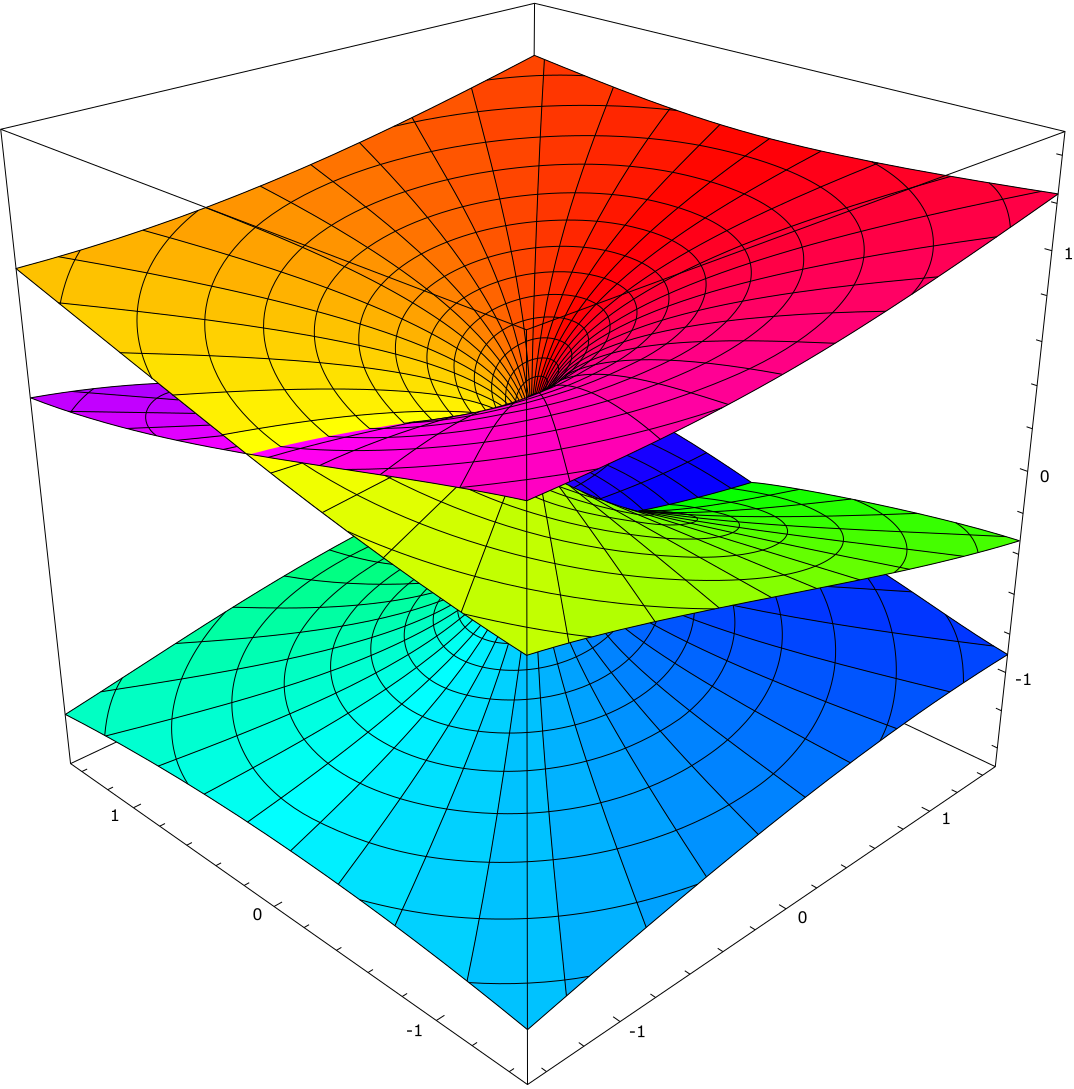
\includegraphics[width=0.4\textwidth]{images/cube_root.png}
    \hfill
    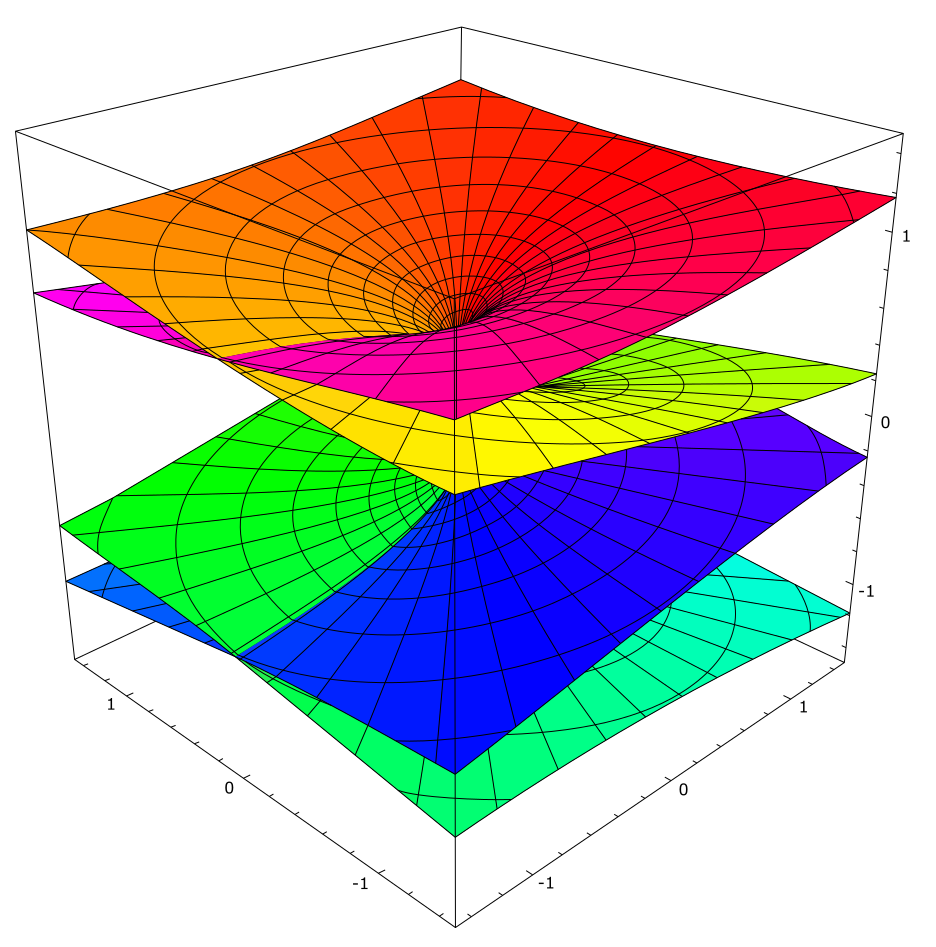
\includegraphics[width=0.4\textwidth]{images/4th_root.png}
    \caption{This is what $z \mapsto z^n$ looks like for $n = 2, 3, 4$ around $z = 0$.}
  \end{figure}

  \begin{figure}
    \centering
    \vspace{5cm}
    \caption{Qualitative diagram of the ramified covering of $f(z) = \dfrac{z^2}{z+1}$. (Caution: Removing ramified points does not disconnect the Riemann sphere. Use this diagram carefully.) }
  \end{figure}

\end{document}
